% BEGIN SECTION 1 - MILAN
% Last updated by Milan Ilnyckyj 2013-08-26


		\singlespacing
		\section{Executive summary}
		\label{sec:ExecutiveSummary}
		\doublespacing



% Has incorporated comments from Mie Inouye, Lauren Sweeney, Alena Prazak, and others



The governments of the world --- including the governments of Canada, the United States, the United Kingdom, China, Brazil, and the 27 European Union members --- have agreed we should avoid raising global temperatures to more than 2˚C above pre-industrial levels.\footcite[][]{CopenhagenAccord}
This is the threshold at which the major governments of the world have agreed that climate change becomes ``dangerous''.
Based on hundreds of thousands of years of evidence on how the climate responds to greenhouse gases (GHGs), we can calculate the total quantity of all fossil fuels we can burn, adding the carbon they contain to the atmosphere, while still giving ourselves a good chance of avoiding a 2˚C increase.\footcite[Research published in \emph{Nature} highlights how even a limit of 2˚C of warming ``is not sufficient to control many other quantities, such as transient sea level rise5, ocean acidification and net primary production on land''. Limiting warming to a lesser level would require even more aggressive action than described in this brief.][p. 197]{Steinacher2013}
To do so we must keep future GHG pollution to no more than 565 billion tonnes (gigatonnes) of carbon dioxide (\ce{CO2}).\footcite[For an more detailed explanation that is accessible to non-experts see: ][]{TerrifyingNewMath}
At the same time, we know that burning the world's proven reserves of coal, oil, and natural gas would produce 2,795 gigatonnes of \ce{CO2} --- nearly five times as much as it would be safe to burn.\footcite[][]{CTI2012} \footcite[Another accessible summary of the issue can be found in this free hour-long radio program: ][]{HotBackyard}
The University of Toronto can play a role in helping humanity stay within these planetary limits, by choosing to sell its investments in fossil fuel companies.



Climate change is a defining example of social injury.
Firms that produce fossil fuels do not bear any economic burden as a result of the many forms of harm they are imposing on other people, including agricultural impacts, sea level rise, damage to human health, and more severe extreme weather.
Likewise, those who use fossil fuels enjoy the benefits while imposing these costs on others.
In order to avoid severe global injury, the total quantity of fossil fuels burned by humanity must be capped at a level far below the level of fossil fuels available to be burned. 
As \emph{The Economist} explains: ``[C]ompanies and governments already have far more oil, gas and coal than they need... assuming temperatures are not to rise by more than 2˚C''.\footcite[][]{EconomistUnburnable}
The International Energy Agency supports this assessment; in their ``2012 World Energy Outlook'' they explain that: ``[n]o more than one-third of proven reserves of fossil fuels can be consumed prior to 2050 if the world is to achieve the 2˚C goal''.\footcite[][p. 25]{IEA2012}
The business plans of fossil fuel companies do not take this reality into account.
They assume they can burn all of their proven reserves, along with any additional reserves they discover in unconventional areas like the arctic, the deep ocean, and Canada's bituminous sands.\footcite[U.S. Energy Information Administration estimates that there are 345 billion barrels of recoverable shale oil around the world, and 7,299 trillion cubic feet of shale gas: ][]{EIAShaleOilGas}
Right now, we are adding over 35 gigatonnes of \ce{CO2} to the atmosphere each year, and the global quantity of that pollution is rising by 3 percent per year.\footcite[][p. 26]{IPCCar4_syr}
That means that we are on track to exceed the 565 gigatonne limit within 15 years.



Two implications arise from this. 
First, we need to meet the world's energy needs while leaving 80 percent of the planet's fossil fuel reserves unburned.\footnote{For reasons of scale and cost, it is not plausible that carbon capture and storage (CCS) will allow us to escape this reality. See: \nameref{CCSSaves}.} 
As NASA climatologist James Hansen explains: ``Rapid reduction of fossil fuel emissions is required for humanity to
succeed in preserving a planet resembling the one on which civilization developed''.\footcite[][]{HansenPaleo}
This requires a massive redirection of investment from funding fossil fuel energy sources to deploying different energy sources that do not alter the climate.\footcite[See: ][]{SternEuropeanLowCarbon}
Second, the stockmarket value of fossil fuel companies is based on the outdated assumption that fossil fuel extraction and use can continue without limit.
If they are allowed to do this, the global effects will be catastrophic.
As such, much of the value of these companies is illusory, based on the out-dated assumption that we can forever use the atmosphere as a free dumping ground for \ce{CO2}.
The energy sources of the future need to be compatible with a stable climate: a fact the investment community has not yet generally accepted, but which they will be confronted with increasingly as the severity of climate change becomes more obvious.
It's time for the smart money to start investing in energy sources that are compatible with a prosperous future, rather than those that threaten to afflict with world with frightening and avoidable harms.



\begin{figure}
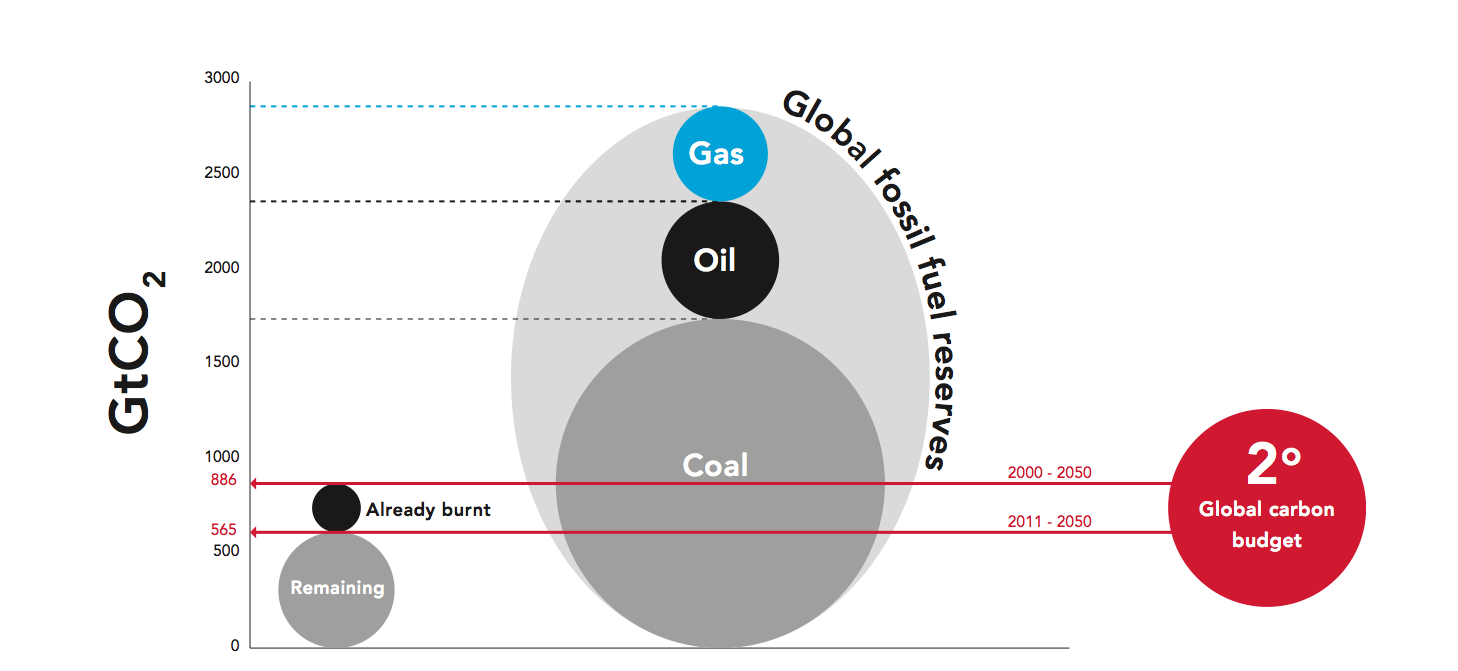
\includegraphics[width=\textwidth]{s1-carbon-budget.png}
\centering
\caption{Comparison of the global 2˚C carbon budget with fossil fuel reserves \ce{CO2} emissions potential. Source: Carbon Tracker Institute, ``Unburnable Carbon: Are the world's financial markets carrying a carbon bubble?'', p. 6}
\label{fig:TwoDegreeBudget}
\end{figure}



Figure \ref{fig:TwoDegreeBudget} from the Carbon Tracker Initiative summarizes the situation in which the world now finds itself, considering the size of fossil fuel reserves and the safe operating parameters of the planet.
On the left are two circles depicting the total `carbon budget' the world can make use of without breaching the ``dangerous'' 2˚C barrier.
The black circle shows what has already been burned and the grey circle shows what could still be burned without breaking the budget limit.
The circles to the right depict the massive quantity of potential \ce{CO2} emissions embedded in the world's remaining coal, oil, and gas.\footcite[][p. 6]{CTI2012}
The world won't be able to shift instantly to zero-carbon forms of energy, but if we are to avoid breaching the limit we have chosen, we need to stop building new fossil-fuel infrastructure that will burden the world for decades and delay investment in forms of energy that can be relied upon indefinitely.
We need to stop funding the worldwide search for unconventional fossil fuel reserves like oil sands, shale gas, and oil under what remains of the arctic ice.
These objectives can be achieved without sacrificing strong financial performance, and while upholding the values of the university. 




\subsection{How the University of Toronto can make a difference}



The International Energy Agency expects \$37 trillion to be spent on energy supply infrastructure between 2012 and 2035.\footcite[][]{IEA2012factsheet}
Humanity must decide whether to spend this money digging ourselves deeper into a pit of fossil fuel dependence, or whether to redirect it toward moving beyond fossil fuels.
The University of Toronto can help lead the necessary redirection of investment that will allow humanity to prevent climatic catastrophe while building a safe and efficient global energy system that can be relied upon indefinitely.
Selling its shares in fossil fuel companies would be an effective way of contributing to this transition.
As with divestment from Apartheid South Africa and the tobacco industry, this choice would make a powerful statement about the kind of future the university wishes to help bring about.
It would also help strip the fossil fuel industry of its social license to operate --- a privilege it is proving unworthy of as it pushes the world heedlessly toward climatic catastrophe while imposing harm on innocent people around the world and in future generations.
By selling its holdings before investors at large accept that most of their reserves are unburnable, the university can mitigate against the risk that fossil fuel stock values will fall substantially as the world realizes that their reserves are too dangerous to burn.



Universities, which collectively have endowments and pension funds worth many billions of dollars, can play an important role in driving this shift toward cost-effective approaches to \ce{CO2} mitigation, including energy conservation and renewable energy deployment.\footcite[The consultancy McKinsey \& Company has studied and ranked global options for mitigating GHG pollution, considering their cost, plausible deployment speed, and the scale at which they can help solve the problem. See: ][p. 8]{McKinseyCurve}
University divestment of fossil fuel company shares would demonstrate that the `smart money' is sufficiently concerned about climate change to take effective action, and could prompt other investors to reconsider their own investment decisions. 
Divestment would help reduce the danger from climate change by decreasing investor confidence in the viability of new projects like coal-fired power plants and oil pipelines.
As the analysis below demonstrates, it could do so while maintaining an overall portfolio with stable and attractive returns.
The legacy of U of T's investments can either be the continued support for projects that clash fundamentally with what we know to be required to preserve a safe climate, or it can be the development and deployment of energy options that are compatible with enduring prosperity for the university and humanity as a whole.



The authors and supporters of this brief call upon the University of Toronto to:
\begin{itemize}
	\item Make an immediate statement of principle, expressing its intention to divest its direct holdings of stock in fossil fuel companies within five years,
	\item Immediately stop making new investments in the industry,
	\item Instruct its investment managers to wind down the university's existing direct stock holdings in the 200 fossil fuel companies listed in \nameref{sec:200Companies} over five years, and
	\item Divest from Royal Dutch Shell by the end of 2013.
\end{itemize}



Divestment from Royal Dutch Shell should be a high priority for the University of Toronto. 
In addition to being a major contributor to climate change, Shell has a continuing history of social injury, both in Canada and around the world. 
As the university's single largest international equity holding, Shell sends the message that the University of Toronto is committed to fossil fuel exploitation and unconcerned about the legal and human rights records of the companies in which it invests. 
Divestment would send the opposite message: that the university is committed to addressing climate change, and willing to start emphasizing that commitment by selling its holding in a particularly problematic investment.  
The university would not suffer financially as a consequence of divesting from Shell and, by doing so, it would protect itself from the risks created by this investment.\footnote{See: \nameref{sec:Shell}}



Across North America, the peer schools of the University of Toronto are considering divestment.
These include Harvard, Yale, Princeton, Stanford, and MIT.
Six schools have already committed to divest.\footnote{For an up-to-date list, see: \url{http://gofossilfree.org/commitments/}}
By leading the way and becoming the first major university to divest, the University of Toronto can distinguish itself as being ahead of the pack on one of the major issues of the 21st century.




The University of Toronto's Statement of Institutional Purpose includes ``a resolute commitment to the principles of equal opportunity, equity and justice''.\footcite{InstitutionalPurpose}
If future generations are to have equal opportunities, they cannot inherit a planet that has been impoverished by uncontrolled climate change.
Similarly, the principles of equity and justice forbid us from ignoring what we know about the harms of GHG pollution by continuing to impose risk and suffering on innocent people around the world and in future generations.
Canada, Toronto, and the University of Toronto have historically benefitted from fossil fuel use far exceeding the global \emph{per capita} average.
Having benefited for decades from behaviour that we now know to be extremely damaging, the university also has a special moral obligation to be part of the solution.



This brief will explain in detail why a decision to divest would improve the financial prospects of the university, uphold its values, and permit the school to take a leadership role in a necessary global transition away from \ce{CO2}-intensive forms of energy. 



% END SECTION 1 - MILAN